%==============================================================================
% Capitulo 7: Resultados
%==============================================================================
\section{Resultados}

Este capítulo presenta los resultados de la validación experimental del sistema. Se reportan los hallazgos en cuatro dimensiones: tiempos de registro, desempeño de clasificación, reducción de la intervención humana y análisis cualitativo de errores.

\subsection{Comparación de tiempos de registro}

La comparación de los tiempos de registro entre el flujo manual y el flujo automatizado se sintetiza en la Tabla~\ref{tab:tiempos}. La media aritmetica del tiempo manual sobre los 200 casos del corpus fue de 61,6~s (mediana de 50,0~s), con un desvio estandar de 44,9~s y un rango entre 10 y 300~s. Este valor, respaldado por la planilla de cronometraje descrita en la Sección~4.2, corresponde a la medición experimental incidente por incidente y reemplaza a la estimación preliminar de 2 minutos con 45 segundos citada en la Sección~1.2, obtenida sin cronometraje individual. La media del flujo automatizado fue de 17,76~s (mediana de 17,47~s), con un desvio estandar de 13,48~s y un rango entre 0,525 y 65,834~s. La reducción relativa de la media de tiempo alcanzó el 71,2~\%.

\begin{table}[htbp]
\centering
\caption{Estadisticos descriptivos de los tiempos de registro por flujo (\(n = 200\))}
\label{tab:tiempos}
\small
\begin{tabular}{@{}>{
aggedright\arraybackslash}p{4.0cm} p{3.5cm} p{3.5cm} p{2.5cm}@{}}
\toprule
\textbf{Estadistico} & \textbf{Flujo manual} & \textbf{Flujo automatizado} & \textbf{Reduccion} \\
\midrule
Media aritmetica (s)      & 61,6   & 17,76   & 71,2~\% \\
Mediana (s)               & 50,0   & 17,47   & 65,1~\% \\
Desvio estandar (s)       & 44,9   & 13,48   & --- \\
Minimo (s)                & 10     & 0,525   & --- \\
Maximo (s)                & 300    & 65,834  & --- \\
\bottomrule
\end{tabular}
\par\smallskip
{\footnotesize\textit{Fuente:} elaboración propia a partir del corpus de validación (\(n = 200\)).\par}
\end{table}

El tiempo automatizado de registro desagregado por canal de origen se presenta en la Tabla~\ref{tab:tiempos-canal}. El canal telefonico incorpora, ademas de la latencia de procesamiento, la duracion de la llamada grabada, de modo que su valor es comparable en su base de medicion con el flujo manual; como la grabacion esta acotada a un maximo de 45~s (véase la Sección~4.4), ese valor constituye una cota inferior de la duracion real de la llamada.

\begin{table}[htbp]
\centering
\caption{Tiempo automatizado de registro por canal de origen (\(n = 200\))}
\label{tab:tiempos-canal}
\small
\begin{tabular}{@{}p{6.0cm} c c c@{}}
\toprule
\textbf{Canal de origen} & \textbf{Casos} & \textbf{Media (s)} & \textbf{Mediana (s)} \\
\midrule
Llamada telefonica (cota inferior) & 81 & 20,09 & 18,70 \\
Correo electronico                 & 66 & 27,65 & 25,82 \\
Formulario web                     & 53 & 1,88  & 1,26  \\
\midrule
\textbf{Global}                    & \textbf{200} & \textbf{17,76} & \textbf{17,47} \\
\bottomrule
\end{tabular}
\par\smallskip
{\footnotesize\textit{Fuente:} elaboración propia a partir del corpus de validación (\(n = 200\)).\par}
\end{table}

La prueba de Wilcoxon de rangos con signo aplicada sobre las mediciones pareadas \parencite{Virtanen2020_scipy} arrojo un estadístico de contraste \(W = \min(T^{+}, T^{-}) = 363\), con una suma de rangos positivos \(T^{+} = 19.737\), una suma de rangos negativos \(T^{-} = 363\) y \(n = 200\) pares validos, junto con un valor \(p = 3{,}08 \times 10^{-32}\), lo que permite rechazar la hipotesis nula de igualdad de medianas con un nivel de confianza superior al 99,9~\%. El estadístico incorpora la corrección por empates y refleja que en 188 de los 200 pares el flujo automatizado fue mas veloz que el manual; en los 12 pares restantes (6,0~\%) el flujo automatizado no fue mas rápido, resultado coherente con la diferencia de aproximadamente 32,5~s entre medianas. La elección de esta prueba no parametrica responde al rechazo de la hipotesis de normalidad en los tres conjuntos de tiempos, cuyo reporte completo se presenta en la Sección~4.7.

Para cuantificar la magnitud práctica de la diferencia, se calculo el coeficiente \(r\) de correlacion rank-biserial a partir de los dos estadísticos de rango:
\[
r = \frac{T^{+} - T^{-}}{n(n+1)/2} = \frac{19.737 - 363}{200 \cdot 201 / 2} = \frac{19.374}{20.100} = 0{,}9639
\]
El valor obtenido (\(r = 0{,}9639\)) corresponde a un tamaño del efecto muy alto, consistente con la alta proporción de pares a favor del flujo automatizado (188 de 200) y con los 12 pares en que este no supero al manual. La diferencia observada es, por tanto, estadísticamente significativa y, dada su magnitud absoluta, relativa y el tamaño del efecto reportado, también prácticamente relevante para la operación.

Cabe señalar que el tiempo manual se registró con redondeo hacia arriba (véase la Sección~4.2), un sesgo de medición sistemático que infla la línea base manual. Por ese motivo la reducción del 71,2~\% debe leerse como cota superior. Un análisis de sensibilidad que descuenta 5~s y 10~s a cada medición manual reduce la media manual a 56,6~s y 51,6~s, respectivamente, y situa la reducción en el 68,6~\% y en el 65,6~\% como cota inferior conservadora. Aun en el escenario mas desfavorable la reducción de tiempo permanece sustancial y estadísticamente significativa (\(p = 1{,}8 \times 10^{-26}\), \(r = 0{,}8683\)).

\begin{figure}[htbp]
\centering
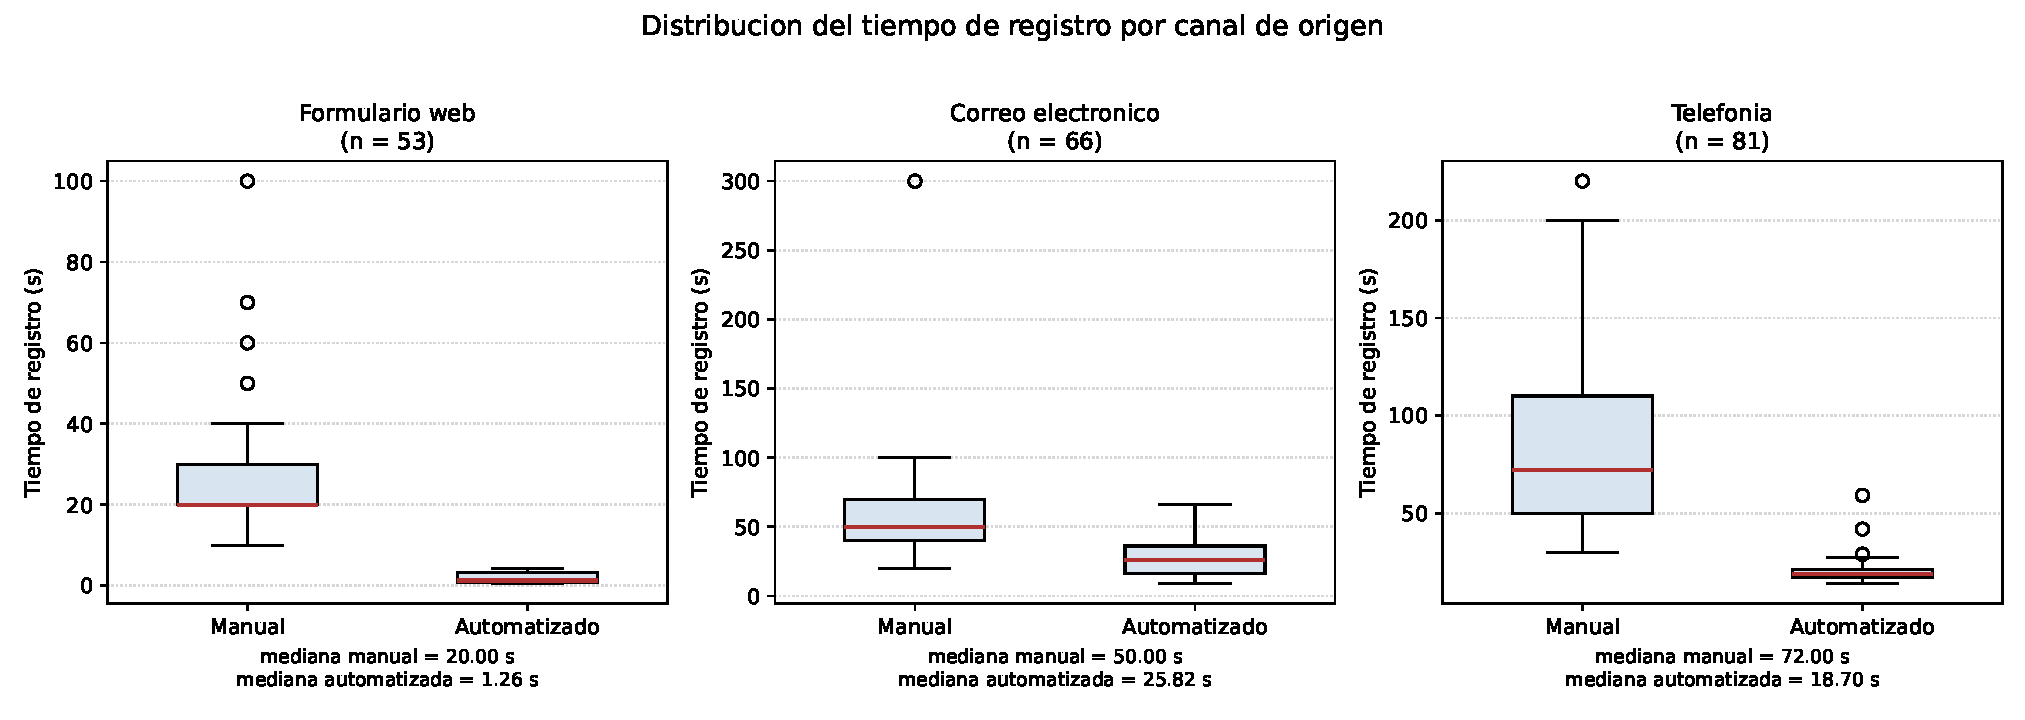
\includegraphics[width=\textwidth]{boxplot_tiempos}
\caption{Distribucion del tiempo de registro por canal de origen (manual frente a automatizado). El panel de telefonia incorpora la duracion de la llamada grabada.}
\label{fig:boxplot_tiempos}
\end{figure}

\subsection{Matriz de confusión y métricas de clasificación}

La evaluación de clasificación se realizó sobre el corpus real de 200 casos pseudonimizados. Su distribución por sector asignado es la siguiente: Soporte Técnico Hardware 85, Soporte Técnico Software 67, Seguridad Informática 31, Sistemas 16 y Bases de Datos 1. Por canal de origen, 81 casos provienen de llamada telefónica, 66 de correo electrónico y 53 de formulario web.

La matriz de confusion obtenida se presenta en la Tabla~\ref{tab:matriz} y en la Figura~\ref{fig:matriz_confusion}. De los 85 casos de Soporte Tecnico Hardware, 77 fueron correctamente clasificados; de los 67 de Soporte Tecnico Software, 48; de los 31 de Seguridad Informatica, 15; de los 16 de Sistemas, 7; y del único caso de Bases de Datos, ninguno. La exactitud estricta resultante asciende al 73,5~\% (147 casos correctos sobre 200).

\begin{table}[htbp]
\centering
\caption{Matriz de confusion del clasificador automatico (\(n = 200\)). Filas: sector asignado; columnas: sector predicho principal.}
\label{tab:matriz}
\small
\setlength{\tabcolsep}{4pt}
\begin{tabular}{@{}>{\raggedright\arraybackslash}p{2.6cm} *{5}{>{\centering\arraybackslash}p{1.85cm}} >{\centering\arraybackslash}p{1.3cm}@{}}
\toprule
\textbf{Asignado \(\backslash\) Predicho} & \textbf{Seguridad Informatica} & \textbf{Soporte Tecnico Hardware} & \textbf{Soporte Tecnico Software} & \textbf{Bases de Datos} & \textbf{Sistemas} & \textbf{Total} \\
\midrule
Seguridad Informatica & 15 & 2 & 11 & 2 & 1 & \textbf{31} \\
Soporte Tecnico Hardware & 1 & \textbf{77} & 3 & 0 & 4 & \textbf{85} \\
Soporte Tecnico Software & 0 & 11 & \textbf{48} & 1 & 7 & \textbf{67} \\
Bases de Datos & 0 & 0 & 1 & 0 & 0 & \textbf{1} \\
Sistemas & 2 & 0 & 5 & 2 & \textbf{7} & \textbf{16} \\
\midrule
\textbf{Total} & \textbf{18} & \textbf{90} & \textbf{68} & \textbf{5} & \textbf{19} & \textbf{200} \\
\bottomrule
\end{tabular}
\par\smallskip
{\footnotesize\textit{Fuente:} elaboración propia a partir del corpus de validación (\(n = 200\)).\par}
\end{table}

\begin{figure}[htbp]
\centering
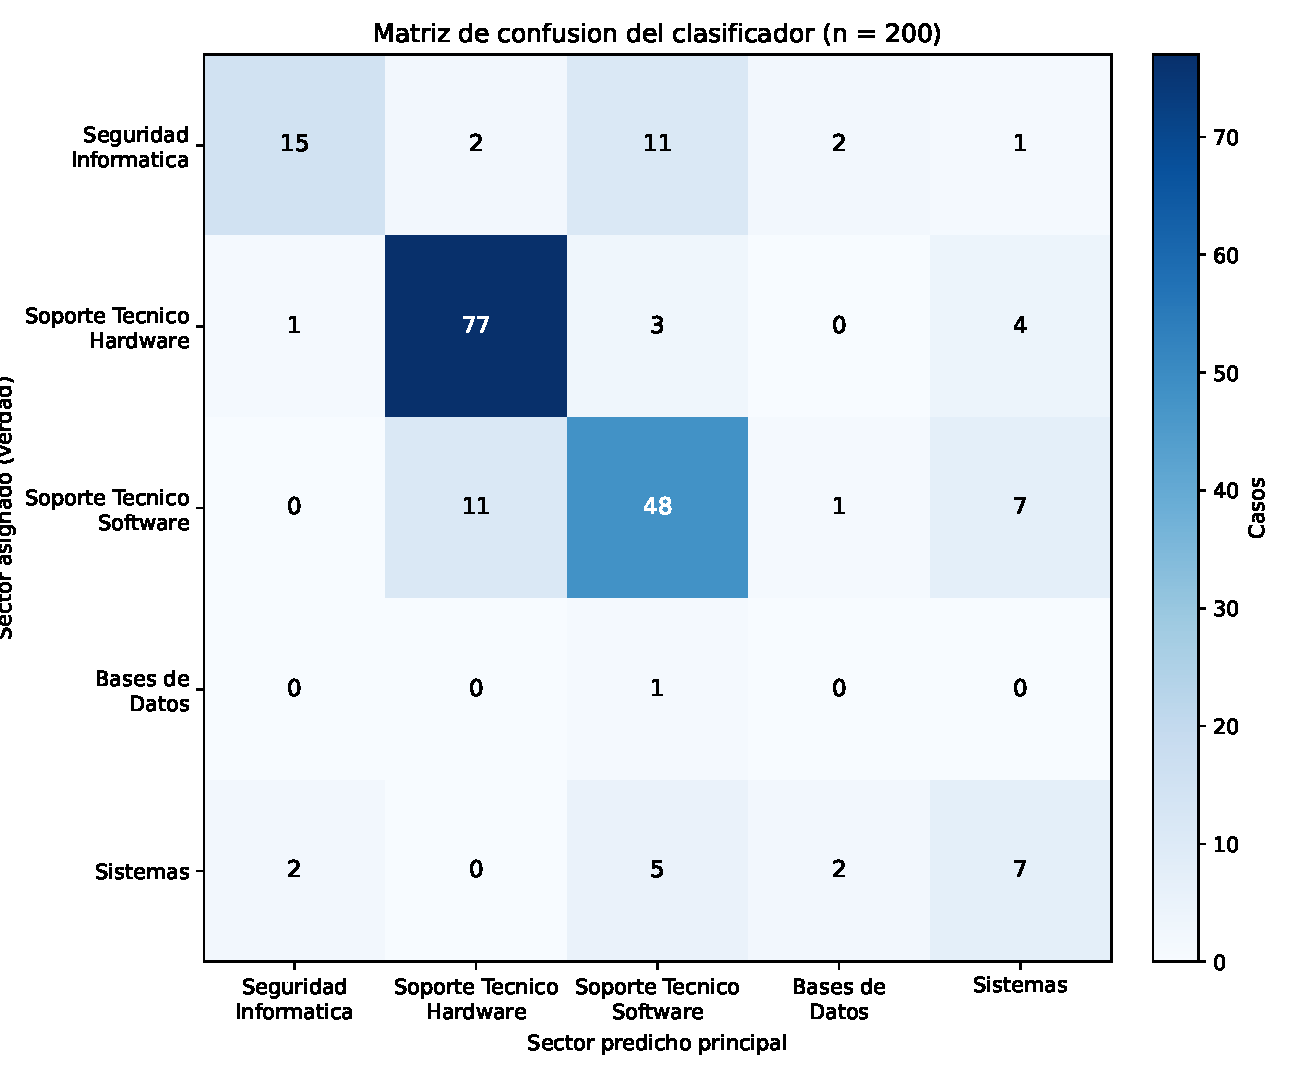
\includegraphics[width=0.85\textwidth]{matriz_confusion}
\caption{Matriz de confusion del clasificador (\(n = 200\)). Filas: sector asignado (verdad); columnas: sector predicho principal.}
\label{fig:matriz_confusion}
\end{figure}

Los valores de precision, sensibilidad (\emph{recall}) y F1 calculados por clase \parencite{Sokolova2009_performance_measures} se presentan en la Tabla~\ref{tab:metricas}. El mejor desempeño correspondió a Soporte Tecnico Hardware (F1 = 0,8800), seguido por Soporte Tecnico Software (0,7111) y Seguridad Informatica (0,6122); Sistemas (0,4000) y Bases de Datos (0,0000, con un único caso de soporte) fueron las clases mas difíciles. El promedio macro de F1 fue de 0,5207 y el micro-F1 de 0,6654. La exactitud estricta del 73,5~\% (147/200) presenta un intervalo de confianza al 95~\%, estimado por el método de Wilson \parencite{Wilson1927_probable_inference}, de [67,0~\%, 79,1~\%]. En cuanto al desempeño de conjunto, el \emph{subset accuracy} (proporción de casos en que el conjunto completo de sectores resultó correcto) fue de 0,43 y el \emph{Hamming loss} de 0,3586. De los 200 casos, 131 fueron resueltos por la etapa determinística del clasificador y 69 requirieron la etapa Gemini.

\begin{table}[htbp]
\centering
\caption{Métricas de clasificación por clase (una contra el resto)}
\label{tab:metricas}
\small
\begin{tabular}{@{}>{\raggedright\arraybackslash}p{4.2cm} >{\centering\arraybackslash}p{2.8cm} >{\centering\arraybackslash}p{2.8cm} >{\centering\arraybackslash}p{2.4cm}@{}}
\toprule
\textbf{Clase} & \textbf{Precision} & \textbf{Sensibilidad} & \textbf{F1} \\
\midrule
Soporte Tecnico Hardware  & 0,8556 & 0,9059 & 0,8800 \\
Soporte Tecnico Software  & 0,7059 & 0,7164 & 0,7111 \\
Seguridad Informatica     & 0,8333 & 0,4839 & 0,6122 \\
Sistemas                  & 0,3684 & 0,4375 & 0,4000 \\
Bases de Datos            & 0,0000 & 0,0000 & 0,0000 \\
\bottomrule
\end{tabular}
\par\smallskip
{\footnotesize\textit{Fuente:} elaboración propia a partir del corpus de validación (\(n = 200\)).\par}
\end{table}

Estas metricas confirman que el clasificador exhibe un desempeño desigual entre las cinco clases objetivo \parencite{Sokolova2009_performance_measures}. La clase mayoritaria (Soporte Tecnico Hardware, con 85 casos) obtuvo el mejor resultado, mientras que Sistemas y Bases de Datos presentaron los valores mas bajos. Este desequilibrio es particularmente relevante en el contexto operativo: un clasificador que concentra sus errores en una clase minoritaria genera derivaciones erroneas en un sector específico, lo que erosiona la confianza de ese equipo en el sistema y puede llevar al rechazo operativo de la herramienta, independientemente de sus metricas agregadas.

La inspeccion de la matriz de confusion revela que los 53 errores totales se concentran en fronteras entre sectores lexicamente proximos, con Soporte Tecnico Software como categoría central. El análisis cualitativo de esos patrones de error, agrupados por frontera de confusion, se desarrolla en la Sección~7.5.

\subsection{Reducción de la intervención humana}

La proporción de intervención humana en el flujo automatizado se calculó a partir de los registros del propio flujo automatizado ---la confianza devuelta por el clasificador en cada caso y las correcciones de categoría introducidas por el sector responsable---, no a partir del instrumento de cronometraje del flujo manual. En el flujo manual, el 100~\% del tiempo correspondio a intervención humana, incluyendo lectura, comprension, busqueda en sistemas auxiliares y carga del ticket. En el flujo automatizado, el operador humano solo intervino en aquellos casos en los que el clasificador devolvio una confianza inferior al 70~\% o en los que el sector responsable, al recibir el ticket, identificó una clasificación incorrecta y la corrigio antes de iniciar la atención.

La proporción de casos con intervención humana en el flujo automatizado se ubico en el 9,5~\%. Este valor es coherente con la propuesta de un esquema \emph{human in the loop} donde el sistema asume la mayoría de los casos rutinarios y reserva al operador la atención de los casos complejos o ambiguos. De los 200 casos procesados, 181 (90,5~\%) fueron clasificados y registrados sin intervención humana, mientras que 19 (9,5~\%) requirieron verificación o corrección por parte de un operador.

\subsection{Calibración de la confianza}
\label{subsec:calibracion}

La confianza declarada por el clasificador solo resulta útil como criterio de derivación si guarda relación con la exactitud real. Para verificar esa relación se contrastó, sobre los 200 casos del corpus, la confianza devuelta en cada predicción contra la corrección de la clasificación. La Tabla~\ref{tab:bandas} desagrega la exactitud por bandas de confianza en torno al umbral del 70~\% que gobierna el gate de revisión humana.

\begin{table}[htbp]
\centering
\caption{Exactitud por banda de confianza declarada}
\label{tab:bandas}
\small
\begin{tabular}{@{}l c c c@{}}
\toprule
\textbf{Banda de confianza} & \textbf{Casos} & \textbf{Aciertos} & \textbf{Exactitud} \\
\midrule
\([0{,}00\,;\,0{,}50)\) & 98 & 75 & 0,765 \\
\([0{,}50\,;\,0{,}70)\) & 26 & 19 & 0,731 \\
\([0{,}70\,;\,0{,}85)\) & 6  & 2  & 0,333 \\
\([0{,}85\,;\,0{,}95)\) & 31 & 22 & 0,710 \\
\([0{,}95\,;\,1{,}00]\) & 39 & 29 & 0,744 \\
\bottomrule
\end{tabular}
\par\smallskip
{\footnotesize\textit{Fuente:} elaboración propia a partir del corpus de validación (\(n = 200\)).\par}
\end{table}

Los datos revelan una calibración invertida o anti-calibrada: los casos de confianza alta (\(\ge 0{,}70\)) fueron menos exactos (0,697) que los de confianza baja (\(< 0{,}70\), 0,758). La tendencia se acentúa en el extremo superior de la escala: dentro de los 46 casos con confianza igual o superior a 0,90 se registraron 13 errores (28,3~\%), y la banda \([0{,}70\,;\,0{,}85)\) alcanzó apenas 0,333 de exactitud. En otras palabras, el clasificador no solo no discrimina mejor cuando declara mayor certeza, sino que en los tramos de confianza mas alta la exactitud se degrada. La consecuencia operativa es directa: el gate del 70~\% ---el mecanismo previsto para derivar a revisión humana los casos dudosos--- no aisló los errores, porque estos se distribuyen también en las bandas de confianza alta. La supervisión humana no puede apoyarse en la confianza declarada como único disparador; requiere complementarse con señales independientes del propio puntaje (por ejemplo, la proximidad léxica entre las categorías candidatas), tal como se discute en el Capitulo~8.

\subsection{Análisis de errores y casos límite}

El análisis cualitativo de los 53 casos mal clasificados permitió identificar patrones de error recurrentes, agrupados por frontera de confusión y sintetizados en la Tabla~\ref{tab:errores}.

\begin{table}[htbp]
\centering
\caption{Confusiones observadas en la clasificación automática, por frontera}
\label{tab:errores}
\small
\begin{tabular}{@{}>{\raggedright\arraybackslash}p{8.5cm} p{2.0cm} p{2.5cm}@{}}
\toprule
\textbf{Frontera de confusion} & \textbf{Casos} & \textbf{Proporcion} \\
\midrule
Soporte Tecnico Hardware \(\leftrightarrow\) Soporte Tecnico Software & 14 & 26,4~\% \\
Sistemas \(\leftrightarrow\) Soporte Tecnico Software & 12 & 22,6~\% \\
Seguridad Informatica \(\leftrightarrow\) Soporte Tecnico Software & 11 & 20,8~\% \\
Otras fronteras & 16 & 30,2~\% \\
\midrule
\textbf{Total} & \textbf{53} & \textbf{100~\%} \\
\bottomrule
\end{tabular}
\par\smallskip
{\footnotesize\textit{Fuente:} elaboración propia a partir del corpus de validación (\(n = 200\)).\par}
\end{table}

El patron dominante, presente en 14 casos (26,4~\% de los errores), corresponde a la frontera entre Soporte Tecnico Hardware y Soporte Tecnico Software: incidentes en que una falla física de un equipo afecta a una aplicación, o en que una tarea sobre una aplicación se describe con terminos de equipamiento, de modo que la decision correcta depende del juicio humano sobre que aspecto prevalece. El segundo patron, presente en 12 casos (22,6~\%), corresponde a la frontera entre Sistemas y Soporte Tecnico Software, asociada a acciones sobre servidores y servicios de plataforma descritas como problemas de una aplicación. El tercer patron, presente en 11 casos (20,8~\%), corresponde a la frontera entre Seguridad Informatica y Soporte Tecnico Software, vinculada a incidentes de acceso y credenciales. El 30,2~\% restante se reparte entre las demas fronteras, incluidas las confusiones que involucran a Bases de Datos, con un único caso de soporte.

Los patrones anteriores se ilustran con tres casos mal clasificados del corpus. Las descripciones se reproducen anonimizadas ---se eliminaron nombres de personas, correos, teléfonos, direcciones y denominaciones internas de sistemas--- y se acompañan con el sector asignado, el sector predicho y la confianza declarada por el clasificador. El primer caso corresponde al patrón de descripción corta: la entrada ``No puede ingresar al sistema central'' fue asignada a Seguridad Informatica y predicha como Soporte Tecnico Software con una confianza de 0,95; su brevedad no aporta contexto sobre el recurso ni sobre la naturaleza del acceso fallido, de modo que la frontera resulta indistinguible sin información adicional. El segundo ilustra la mezcla de categorías: ``Su equipo se reinicia de forma reiterada; el usuario sospecha de los cables'' fue asignada a Soporte Tecnico Software y predicha como Soporte Tecnico Hardware con 0,50 de confianza, y combina un síntoma de nivel de aplicación con una hipótesis de causa física cuyo peso relativo no queda determinado por el texto. El tercero ejemplifica la jerga local: ``No le salen los correos por el flujo interno y no le llegan las instancias'' fue asignada a Sistemas y predicha como Soporte Tecnico Software con 0,85 de confianza, y apela a términos organizacionales (``flujo'', ``instancias'') cuyo significado no está disponible para el clasificador. En los tres casos la confianza declarada es alta pese al error, lo que refuerza el problema de calibración descrito en la Sección~\ref{subsec:calibracion}.

Esta tipologia orienta directamente las recomendaciones presentadas en el Capitulo~10, particularmente la incorporacion de un clasificador supervisado entrenado con el corpus etiquetado generado por el propio sistema y la inclusion de un glosario de terminos organizacionales en el prompt del modelo.

\newpage
